\documentclass[11pt]{article}
\usepackage[utf8]{inputenc}
\usepackage[margin=1in]{geometry}
\usepackage{float}

\usepackage{graphicx}
\graphicspath{{images/}}

\newcommand{\glossaryentry}[2]{#1 - #2}

\setlength{\parskip}{1em}
\setlength{\parindent}{0em}

\title{A Comparison of Immutable and Mutable Data Structures}
\author{}
\date{}

\begin{document}

\maketitle

\begin{center}
By:  Chi Jon, Daniil Furmanov, and Justin Harrison

\hfill

Submitted to Jordan Berard,

In partial fulfillment of the requirements of ENL1813T

\hfill

Algonquin College,

Computer Engineering Technology

\hfill

April 1, 2016

\clearpage
\end{center}

\section*{Glossary}
\glossaryentry{Data Structure}{
  A format to efficiently store information. A common data
  structure is the array, where data is stored sequentially in memory.
}

\glossaryentry{Immutable Data Structure}{
  A data structure that cannot be modified in-place.
  Instead, a new copy with the modifications is created.
}

\glossaryentry{Mutable Data Structure}{
  A data structure that can be modified in-place.
}
\clearpage

\section*{Introduction}
The purpose of this comparison is to determine which type of data structure,
immutable or mutable, is best for a range of programming problems.

For most of the history of Computer Science, mutability has been the standard.
However, with the rise of functional languages, immutability has been gaining
traction \cite{ieee_spectrum}. With this report, we'll hopefully be able to
understand the benefits of immutable and mutable data structures. Which will
give us insight into what is causing the growth of immutability.

This report will compare the differences between immutable and mutable data
structures, using the following three criteria: performance, ease of use, and
safety.

Computer Engineering and Computer Science students will find this report useful,
due to the crucial importance of data structures in our programs.
\clearpage

\section{Performance}
\subsection{Immutable Data Structures}
Immutable data structures have a reputation of low-performance, but this is not
exactly true in the modern-age. With the rise of multi-core consumer devices,
many of the performance short-falls have been removed, and in fact, became
advantages \cite{slaks}.

When sharing a mutable data structure across many threads, the programmer must
use a lock to prevent modifications from conflicting. Locks are theoretically
cheap when it comes to performance, but practically are expensive
\cite{attractive_chaos}.

Immutable data structures in comparison doesn't need the use of atomic locks.
Instead, each thread modifies a section of the structure, with a "master"
thread combining those changes when ready.

For example, let's say there's an immutable string containing the letter 'a'.
If you wanted to change the string to contain 'ab', you'd need to make a whole
new string object containing 'ab'. An example of this can be seen in figure 1.

\begin{figure}[H]
\centering

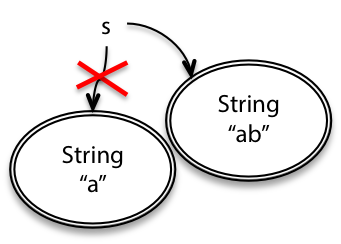
\includegraphics{immutable_string}
\caption{Memory of an immutable string \cite{mit_reading_9}}

\end{figure}

As you can see, immutability has many performance benefits when using multiple
threads. Therefore, immutable data structures are very efficient when used in a
multi-core environment, which most consumer and enterprise devices fit into.

\section{Ease of Use}
\subsection{Immutable Data Structures}
Immutable data structures fall short when it comes to ease of use. Since these
data structures by very definition can't directly be modified, the programmer
must take take great care when using an immutable data structure.

Most programmers are used to object-oriented programming, where mutability has
become the default. In contrast, functional programming has immutablity as
default \cite{miles}. Thefefore, the ease of use depends on which style of
programming you're used to.

However, since the object-oriented style of programming dominates many areas
of software development, it can be said that immutablity doesn't have an
advantage in ease of use for the majority of programmers \cite{ieee_spectrum}.

\subsection{Mutable Data Structures}
One of the main advantages of using mutable structures is that it is much
easier to create a bug-free code than immutable structure. Our perception of
reality is based on mutable objects.  For example, when we fill up a glass of
water, we perceive it as the same object all long.  Its identity remains the
same but its state changes.  It is not the case that we replace the old glass
with new one and fill up with water.  Therefore, when we are modeling a
real-world domain, it makes more sense to use mutable data structures
\cite{peter_toro}.

\begin{figure}[H]
\centering

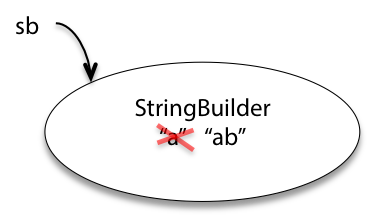
\includegraphics{string_builder}
\caption{Memory of Java's StringBuilder \cite{mit_reading_9}}

\end{figure}

\section{Safety}
\clearpage

\begin{thebibliography}{9}

\bibitem{ieee_spectrum}
  Nick Diakopoulos and Stephen Cass,
  "Interactive: The Top Programming Languages 2015"
  IEEE Spectrum.
  2015
  [Online].
  Available: http://spectrum.ieee.org/static/interactive-the-top-programming-languages-2015
  [Accessed 03 April 2016]

\bibitem{slaks}
  Schabse Laks,
  "Immutability, part 3: Writing thread-safe data structures"
  Slaks Blog.
  2013.
  [Online].
  Available: http://blog.slaks.net/2013-07-22/thread-safe-data-structures/
  [Accessed 03 April 2016]

\bibitem{attractive_chaos}
  AttractiveChaos,
  "Multi-threaded programming: efficiency of locking"
  Attractive Chaos.
  2011.
  [Online].
  Available: https://attractivechaos.wordpress.com/2011/10/06/multi-threaded-programming-efficiency-of-locking/
  [Accessed 08 April 2016]

\bibitem{miles}
	Vagif Abilov
	"Why care about functional programming? Part 1: Immutability"
	2013
	[Online].
	Available: http://miles.no/blogg/why-care-about-functional-programming-part-1-immutability
	[Accessed 10 April 2016]

\bibitem{peter_toro}
	Peter Toro,
	“If immutable objects are good, why do people keep creating mutable objects?”
	2012.
	[Online].
	Available: http://programmers.stackexchange.com/questions/151733/if-immutable-objects-are-good-why-do-people-keep-creating-mutable-objects.
	[Accessed 03 April 2016]

\bibitem{mit_reading_9}
	MIT
	"Reading 9: Mutability and Immutability"
	2015.
	[Online].
	Available: http://web.mit.edu/6.005/www/fa15/classes/09-immutability/
	[Accessed 10 April 2016]

\end{thebibliography}

\end{document}
